\documentclass[12pt]{article}

\usepackage{url,graphicx,amssymb,lastpage}

\usepackage[usenames,dvipsnames,table]{xcolor}

\usepackage{listings}
\definecolor{codegreen}{rgb}{0,0.6,0}
\definecolor{codegray}{rgb}{0.5,0.5,0.5}
\definecolor{codepurple}{rgb}{0.58,0,0.82}
\definecolor{backcolour}{rgb}{0.95,0.95,0.92}
\lstdefinestyle{mystyle}{
    backgroundcolor=\color{backcolour},   
    commentstyle=\color{codegreen},
    keywordstyle=\color{magenta},
    numberstyle=\tiny\color{codegray},
    stringstyle=\color{codepurple},
    basicstyle=\footnotesize,
    breakatwhitespace=false,
    breaklines=true,
    captionpos=b,
    keepspaces=true,
%     numbers=false,
    numbersep=5pt,
    showspaces=false,
    showstringspaces=false,
    showtabs=false,
    tabsize=2
}
 
\lstset{style=mystyle}
 


\usepackage{soul}
\setuldepth{a}

\usepackage{cmbright}
\usepackage[T1]{fontenc}

\usepackage[normalem]{ulem}

\usepackage{fancyhdr}

\pagestyle{fancy}
\renewcommand{\headrulewidth}{0pt}
% \fancyhead[LEO]{\textcolor[gray]{0.4}{Neil Vaytet \hfill \acronym -- Standard EF}}
\fancyhead[CEO]{\textcolor[gray]{0.4}{Plotting-Ramses User Guide}}
% \fancyfoot[LEO]{\textcolor[gray]{0.4}{H2020-MSCA-IF-2014-Standard EF \hfill Part B -- Page \thepage ~of \pageref*{LastPage}}}
\fancyfoot[CEO]{\textcolor[gray]{0.4}{Page \thepage ~of \pageref*{LastPage}}}
% \fancyfoot[LEO]{\textcolor[gray]{0.4}{Neil Vaytet \hfill Part B -- Page \thepage ~of \pageref*{LastPage}}}

% \cfoot{}
\rhead{}
\lhead{}
% \renewcommand{\contentsname}{\hfill TABLE OF CONTENTS \hfill}

\usepackage[pdftex]{hyperref}
\hypersetup{colorlinks=true,linkcolor=black,citecolor=blue,urlcolor=blue}
\urlstyle{sf}

\topmargin -0.40in
\textheight 9.0in
\oddsidemargin 0.0in
\evensidemargin 0.0in
\textwidth 6.5in
% \headsep 12pt
% \footskip 18pt

\setlength\headwidth{\textwidth}

%%%%%%%%%%%%%%%%%%%%%%%%%%%%%%%%%%%%%%%%%%%%%%%%%%%%%%%%%%%%%%%%%%%%%%%%%%%%%%%%%%%%%%%%%%%%%%%%%%%%%
%%%%%%%%%%%%%%%%%%%%%%%%%%%%%%%%%%%%%%%%%%%%%%%%%%%%%%%%%%%%%%%%%%%%%%%%%%%%%%%%%%%%%%%%%%%%%%%%%%%%%
%%%%%%%%%%%%%%%%%%%%%%%%%%%%%%%%%%%%%%%%%%%%%%%%%%%%%%%%%%%%%%%%%%%%%%%%%%%%%%%%%%%%%%%%%%%%%%%%%%%%%

\begin{document}

\begin{center}
\huge

\vspace*{50pt}

\textbf{Plotting-Ramses\\User Guide}

\thispagestyle{empty}

\vspace{50pt}

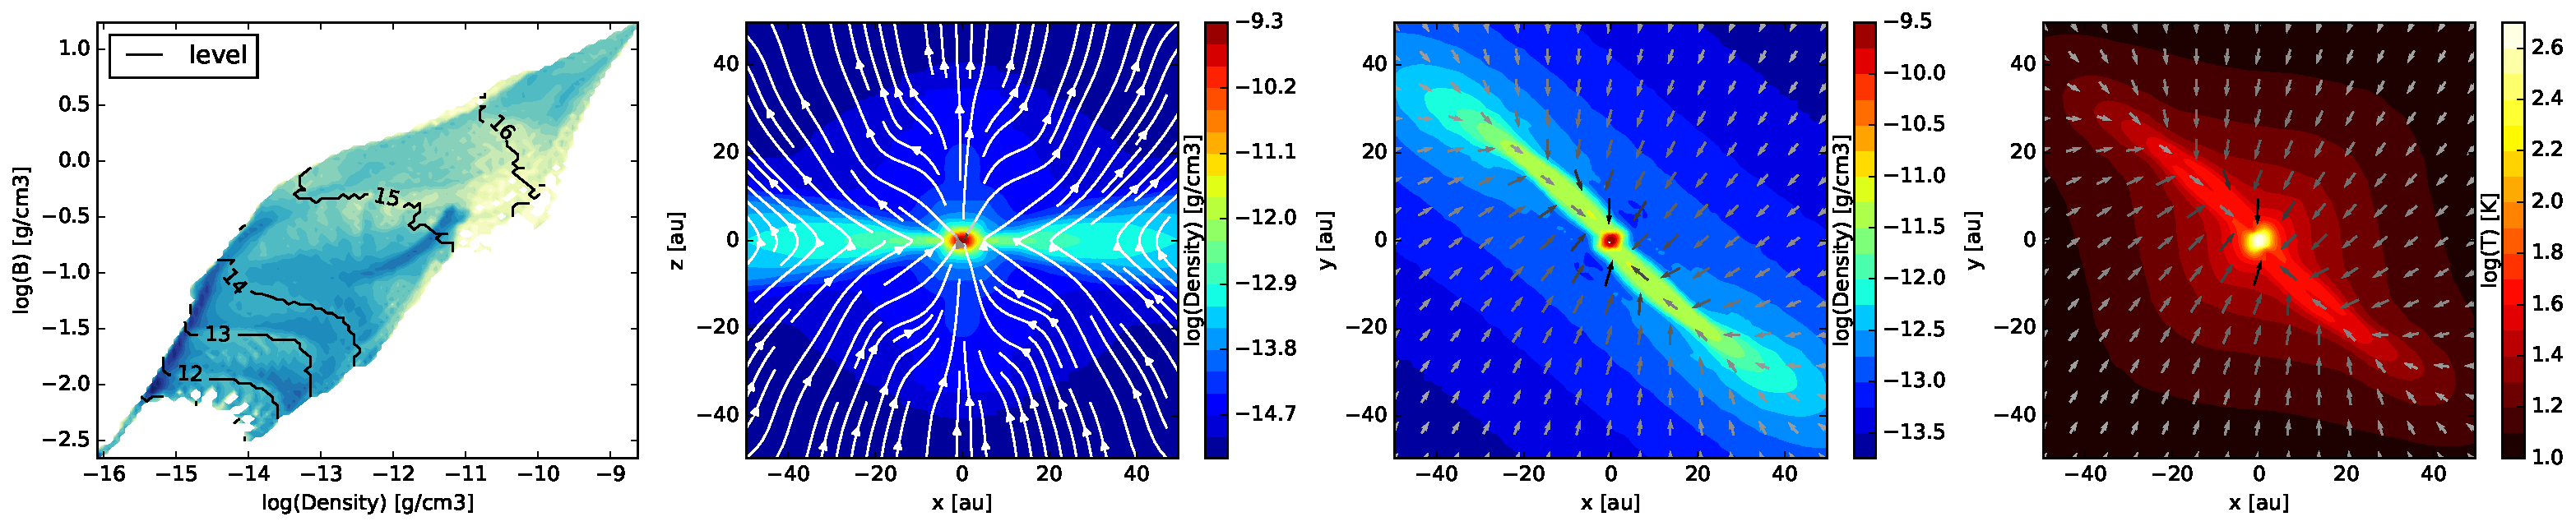
\includegraphics[width=\textwidth]{demo.pdf}

\Large

\vspace{100pt}

Neil Vaytet

\vspace{5pt}

Centre for Star and Planet Formation\\
Niels Bohr Institute\\
University of Copenhagen\\
Denmark

\vspace{5pt}

\textcolor{blue}{\texttt{neil.vaytet@nbi.ku.dk}}

\vspace{70pt}

Version 1.0 - 18/03/2017

\end{center}

\clearpage

\tableofcontents

\clearpage



\section{Introduction}

Plotting-Ramses was developed to provide a light-weight method to read and plot basic diagnostics on \href{https://bitbucket.org/rteyssie/ramses}{\texttt{RAMSES}} simulation outputs. It currently only works with the native `binary' data output format. It uses \texttt{f2py} to interface a fast \texttt{Fortran90} file reader with a \texttt{Python-matplotlib} layer for data manipulation and visualization.

\section{Getting started}

You will need matplotlib and f2py installed on your system.
Before plotting, you must first run 'f2py' on the fortran subroutine which reads in the RAMSES data:

\begin{lstlisting}
f2py -c read_ramses_data.f90 -m read_ramses_data
\end{lstlisting}


\section{Getting help}

Plotting-Ramses was developed by Neil Vaytet \& Tommaso Grassi from the Centre for Star and Planet Formation, at the University of Copenhagen, Denmark.

\noindent The software is free for anyone to use, but absolutely no warranty is provided. If you run into bugs or issues, you can contact the authors via email at \textcolor{blue}{\texttt{neil.vaytet@nbi.ku.dk}}.

\end{document}

